\documentclass[conference]{IEEEtran}
\IEEEoverridecommandlockouts
% The preceding line is only needed to identify funding in the first footnote. If that is unneeded, please comment it out.
\include{../solutions}
\usepackage{cite}
\usepackage{amsmath,amssymb,amsfonts}
% \usepackage{algorithmic}
\usepackage{graphicx}
\usepackage{textcomp}
\usepackage{float}
\usepackage{xcolor}
\usepackage{tabularx}
\usepackage{hyperref}

\hypersetup{
    colorlinks=true,
    linkcolor=blue, 
    citecolor=red,
    filecolor=magenta,
    urlcolor=cyan,
    anchorcolor=black
}

\def\BibTeX{{\rm B\kern-.05em{\sc i\kern-.025em b}\kern-.08em
    T\kern-.1667em\lower.7ex\hbox{E}\kern-.125emX}}

\title{\LARGE{Radiogenomic Prediction of Breast Cancer Subtypes \\ Using the TCGA Dataset}}

\author{
    \begin{tabular}{c}
        \begin{tabular}{cc}
            \begin{tabular}{c} 
                \IEEEauthorblockN{Lucas Fayolle} \\
                \vspace{-8mm}
                \IEEEauthorblockA{\textit{lfayoll@etsinf.upv.es}}
            \end{tabular} &
            \begin{tabular}{c} 
                \vspace{-4.5mm}
                \IEEEauthorblockN{Jose Valero Sanchis} \\
                \vspace{-8mm}
                \IEEEauthorblockA{\textit{jvalsan@etsinf.upv.es}}
            \end{tabular}
        \end{tabular}
    \end{tabular}
}

\begin{document}

\maketitle

\begin{abstract}
Breast cancer subtype classification is essential for guiding personalized treatments. While molecular profiling provides valuable insights, these tests can be costly and invasive. Radiomics offers a non-invasive alternative by extracting quantitative features from MRI images that capture tumor characteristics. 

This study develops machine learning models to predict breast cancer molecular subtypes using radiomic features and evaluates the impact of incorporating clinical and genomic data. The model combining radiomic features + clinical data (including hormone receptor status) achieved the highest performance, with a macro F1-score of 0.78. Additionally, the integration of genomic data improved model performance, demonstrating the complementarity between radiomic and genomic features. These findings highlight the potential of combining imaging, clinical, and genomic data to improve subtype classification.
\end{abstract}

\begin{IEEEkeywords}
Breast cancer, radiomics, machine learning, molecular subtypes, genomic assays, clinical data, MRI.
\end{IEEEkeywords}

%%%%%%%%%%%%%%%%%%%%%%%%%%%%%%%%%%%%%%%%%%%%%%%%%%%%%%%%%%%%%%%%%%%%%%%%%%%%%%%
%                                                                                          INTRODUCTION                                                                                                                   %
%%%%%%%%%%%%%%%%%%%%%%%%%%%%%%%%%%%%%%%%%%%%%%%%%%%%%%%%%%%%%%%%%%%%%%%%%%%%%%%

\section{Introduction}

\subsection{Background and motivation}

Breast cancer is one of the most common cancers worldwide and a leading cause of mortality among women \cite{breast_cancer}. Molecular profiling has identified subtypes such as Luminal A, Luminal B, HER2-enriched, and Basal-like, which are essential for guiding personalized treatments \cite{b1}. However, determining these subtypes often requires invasive procedures, such as biopsies and genomic assays, which can be costly and time-consuming.

Radiomics offers a non-invasive approach by extracting quantitative features from MRI images that can capture tumor phenotypic traits linked to molecular profiles. Integrating radiomic features with clinical and genomic data can enhance machine learning models for breast cancer subtype prediction. \cite{b2}

This project aims to develop a classifier that predicts molecular subtypes based on MRI-derived radiomic features and evaluates the impact of incorporating clinical and genomic data to improve performance.

\subsection{Project objectives}

The primary objective of this project is to develop a machine learning classifier capable of predicting the molecular subtypes of breast cancer (Luminal A, Luminal B, HER2-enriched, Basal-like) using radiomic features extracted from MRI images.

To achieve this, the following specific objectives are proposed:

\begin{itemize}
	\item \textbf{Utilization of the provided radiomic features}. A preprocessing pipeline will be applied to the radiomic data provided, incorporating feature selection methods, such as Boruta, to refine the input features. Once processed, the machine learning models will be trained and evaluated using relevant performance metrics to assess their predictive accuracy.

	\item \textbf{Incorporation of clinical data}. Clinical variables, such as age and tumor stage, will be integrated into the dataset. Models trained with this comprehensive feature set will be compared to previous models to evaluate the impact of clinical data on predictive performance.	

	\item \textbf{Integration of multigenic assay data}. Multigenic assay scores will be analyzed for correlations with radiomic features and added as predictors. Models will be trained with the extended dataset, and their performance will be assessed to determine if genomic data enhances prediction.
\end{itemize}

\subsection{Report structure}

This report is organized into five main sections. The Introduction presents the background, motivation, and objectives of the study. The Methodology describes the datasets used, the data preprocessing steps, and the exploratory data analysis, followed by the feature selection. The Model development section explains the different machine learning models created and the evaluation metrics used to assess their performance. The Results and discussion section compares the models' performance and analyzes the impact of incorporating clinical and genomic data. Finally, the Conclusions summarize the key findings, discuss limitations, and propose future work.

%%%%%%%%%%%%%%%%%%%%%%%%%%%%%%%%%%%%%%%%%%%%%%%%%%%%%%%%%%%%%%%%%%%%%%%%%%%%%%%
%                                                                                              Methodology                                                                                                                   %
%%%%%%%%%%%%%%%%%%%%%%%%%%%%%%%%%%%%%%%%%%%%%%%%%%%%%%%%%%%%%%%%%%%%%%%%%%%%%%%

\section{Methodology}

\subsection{Description of datasets}


The data used in this project was obtained from the TCGA Breast Radiogenomics collection available in \cite{b3}. Among other files, such as the original MRI images and their corresponding tumor segmentations (as shown in Figure \ref{fig:mri_example}, illustrating the type of imaging data from which radiomic features are extracted for analysis), the dataset includes three types of data sources: radiomic features, multigenic assay results, and clinical data:

\begin{itemize}
	\item \textbf{Quantitative Radiomic Features}.  This dataset includes 41 quantitative features derived from MRI images, which describe different aspects of the tumor, such as shape, texture, and signal enhancement dynamics.

	\item \textbf{MammaPrint, Oncotype DX, and PAM50 multi-gene assays}. This dataset provides genomic scores associated with breast cancer prognosis and subtype classification. The variable \textbf{Pam50.Call} serves as the target variable, indicating the molecular subtype for each sample.

	\item \textbf{Clinical data}. This dataset contains information on patient demographics, tumor characteristics, and treatment-related variables

\end{itemize}

\begin{figure}
    \centering
    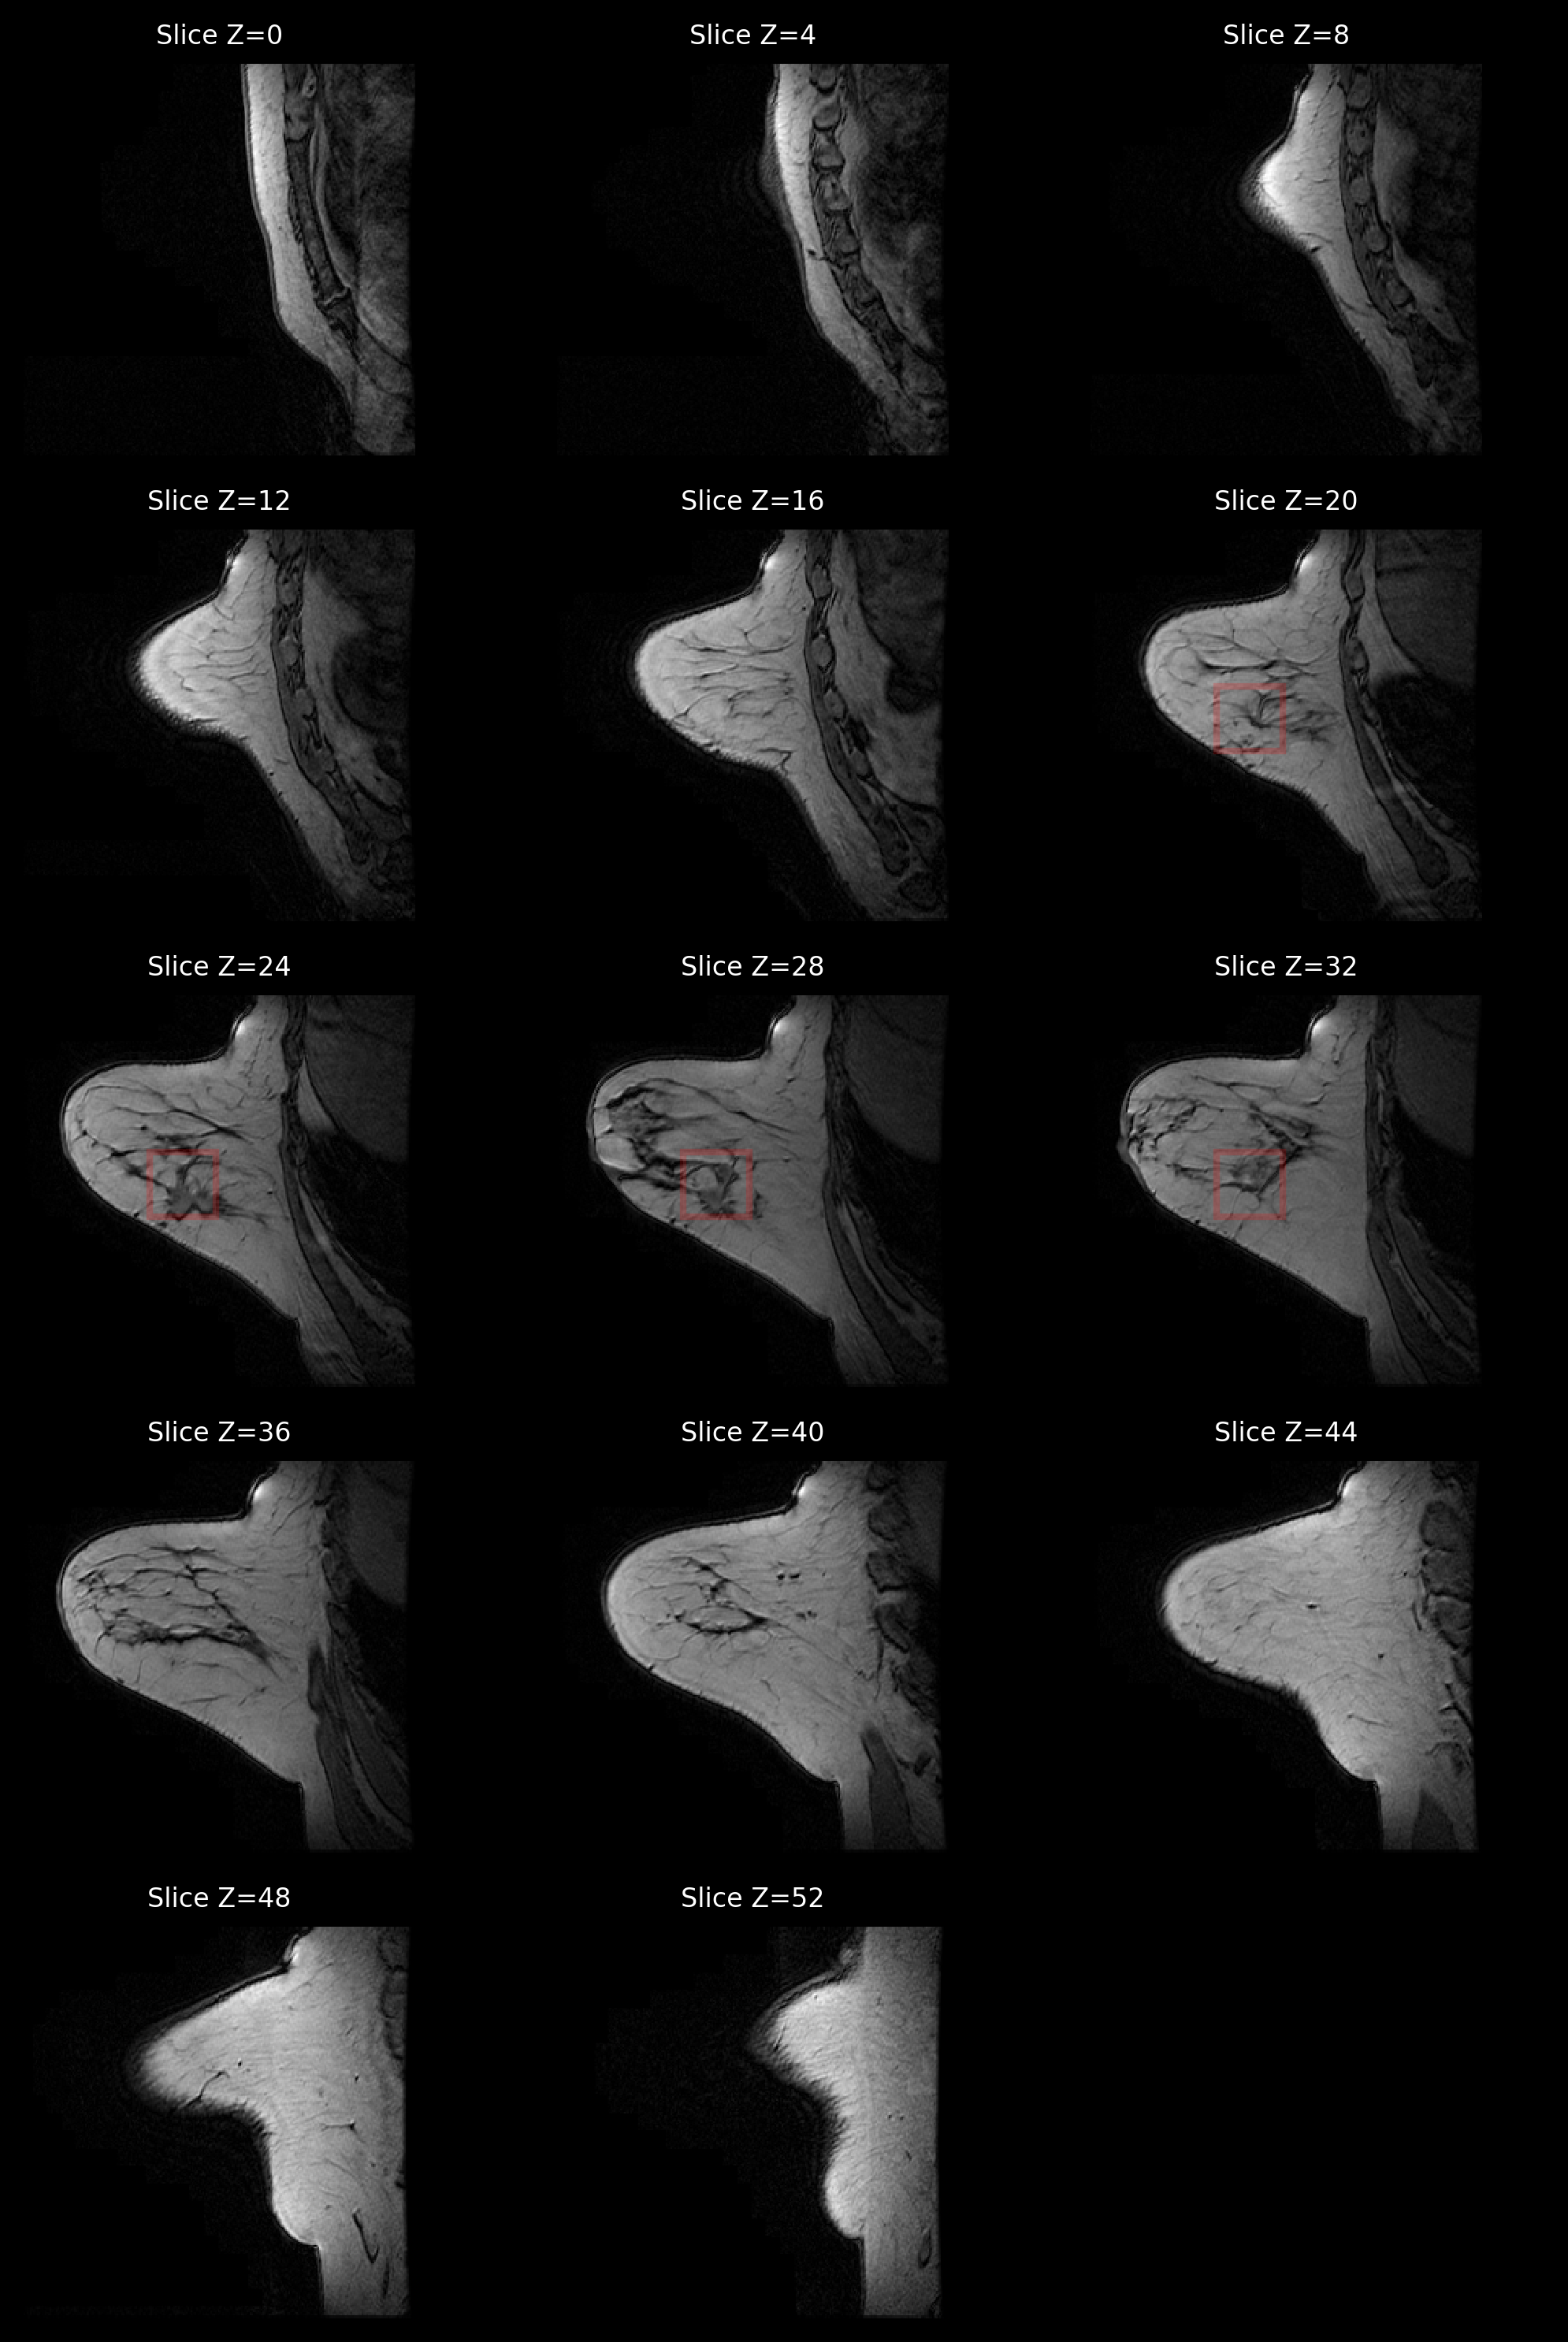
\includegraphics[width=0.45\textwidth]{images/mri_example.png}
    \caption{Example MRI scan with corresponding tumor segmentation}
    \label{fig:mri_example}
\end{figure}

\subsection{Data preprocessing}

The data preprocessing phase ensures that the dataset is consistent and focused on the relevant classification task by selecting complete instances and excluding irrelevant categories.

\subsubsection{Identification of complete instances}

In this step, we ensure that only instances with complete information across all datasets—radiomic features, multigenic assay results, and clinical data—are included. This guarantees that the training and evaluation of machine learning models are performed consistently with the same set of data points, regardless of the features being tested.

The approach involves checking for the presence of a common identifier (CLID) across the three datasets. Instances that do not have corresponding entries in the radiomic, multigenic, or clinical datasets are excluded.

As a result, a new dataset containing only the complete instances is created, ensuring uniformity in the data used across all experiments.

\subsubsection{Removal of the ``normal" category}

In this step, instances labeled as ``Normal" in the Pam50.Call variable are excluded from the dataset. The rationale behind this decision is that the focus of the project is to differentiate between molecular subtypes of breast cancer, not to distinguish between healthy and cancerous tissue. Including ``Normal" as a class would introduce a category that lacks clinical relevance for the subtype prediction task, as ``Normal" does not correspond to a specific cancer phenotype.

\vspace{5mm}

After this preprocessing, from the 84 cases present in the original dataset, 76 instances remain for analysis in this project. The distribution of the target variable in these instances is shown in Figure \ref{fig:pam_distr}.

\begin{figure}[H]
    \centering
    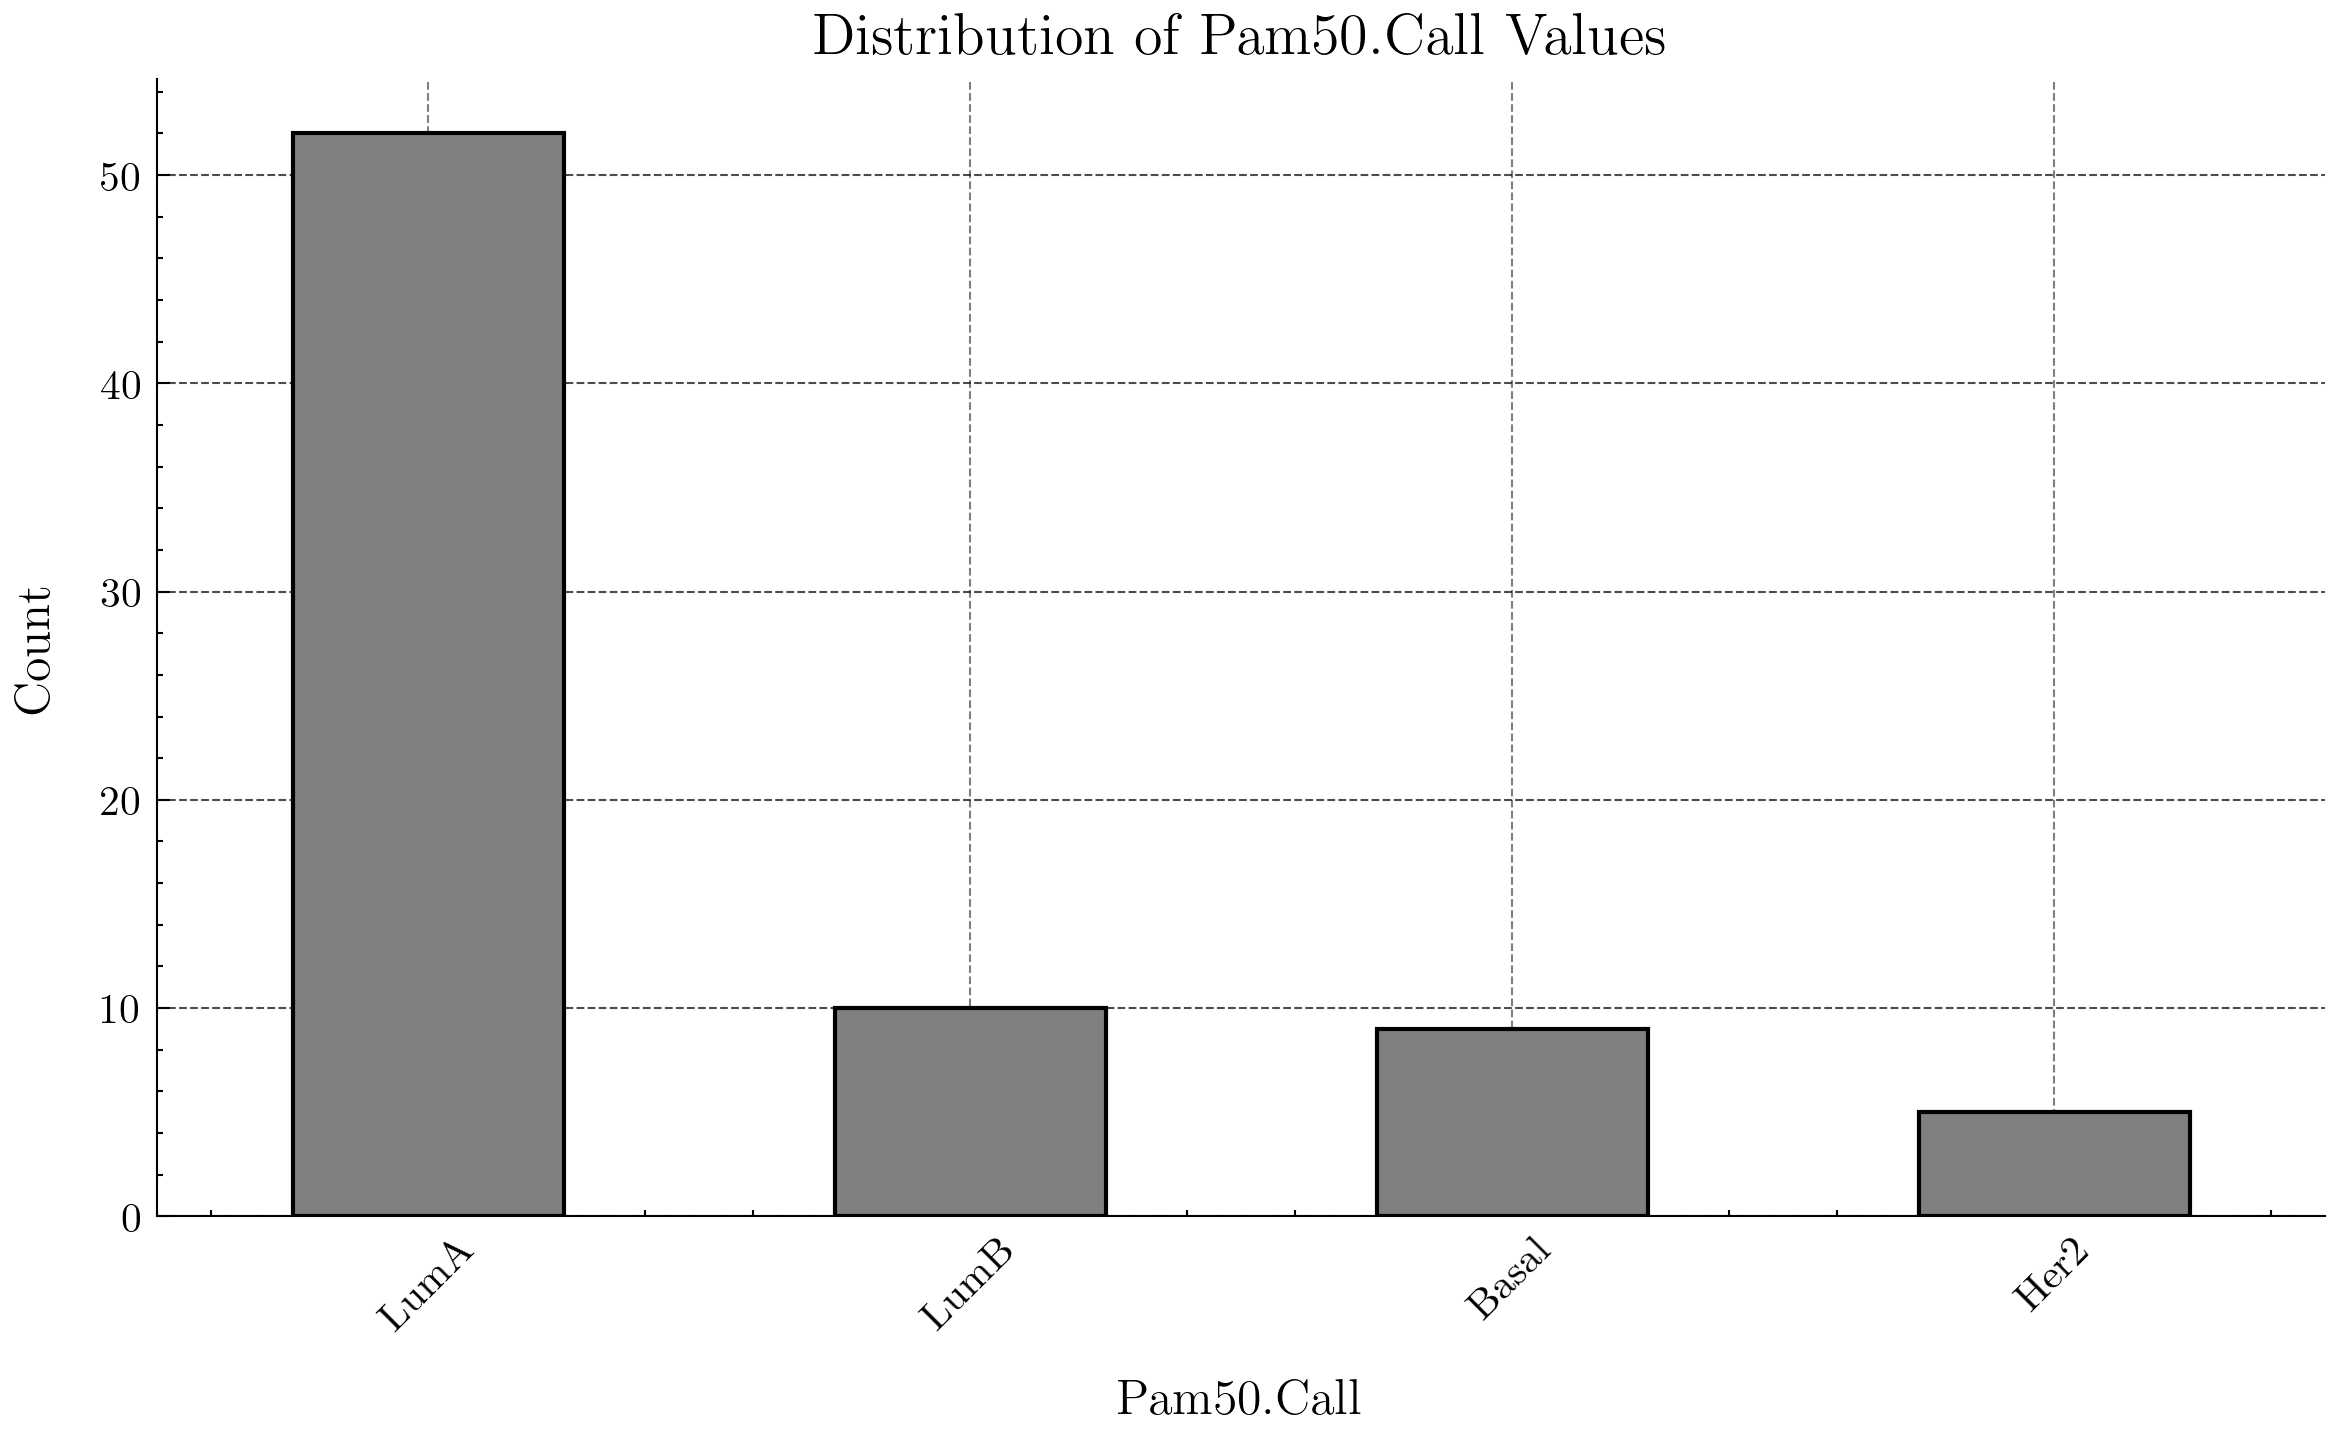
\includegraphics[width=0.5\textwidth]{images/pam_distr.png}
    \caption{Distribution of \texttt{Pam50.Call} values}
    \label{fig:pam_distr}
\end{figure}

As shown in the abovementioned figure, there is a significant class imbalance, with the Luminal A subtype being highly overrepresented compared to the other classes. This imbalance must be taken into account when selecting the evaluation metrics for the model. Additionally, as will be discussed in Section \ref{pre-models}, undersampling and oversampling techniques will be applied to address this issue and improve the model’s robustness.

\subsection{Exploratory data analysis (EDA) and feature selection}

The exploratory data analysis (EDA) provides insights into the clinical data and multigenic assay scores, helping to understand their distribution, correlations, and relevance to the target variable. In addition to statistical findings, medical considerations are taken into account to ensure that the selected variables are not only informative but also clinically meaningful for inclusion in the model.

\subsubsection{Clinical data}

The clinical variables included in the model are the patient's age at the time of diagnosis, the cancer's overall stage and tumor size, the number of lymph nodes affected, and the status of estrogen and progesterone receptors. Although an exploratory analysis was conducted to better understand the data distribution, due to space limitations, these details are not displayed. Therefore, the selection of variables is primarily based on clinical criteria:

\begin{itemize}
    \item \textbf{Age at diagnosis}. A key prognostic factor, as younger patients often have more aggressive tumors, while older patients may present less aggressive subtypes. \cite{b4}
    \item \textbf{Cancer stage and tumor size}. These variables describe the extent of disease progression and are crucial for predicting molecular subtypes.
    \item \textbf{Number of affected lymph nodes}.  Indicates metastatic spread and reflects the severity of the disease. \cite{b5}
    \item \textbf{Hormone receptor status (estrogen and progesterone)}. These statuses are essential for distinguishing Luminal subtypes \cite{b6}. However, due to their high correlation with the target variable, a model was also built without them to avoid redundancy.
\end{itemize}

The HER2 receptor status based on immunohistochemistry results was excluded due to a high proportion of missing values, despite its relevance to the HER2-enriched subtype.

\subsubsection{Multigenic assay scores}

The following multigenic assay variables were selected based on their relevance to tumor biology and their ability to complement the radiomic data:

\begin{itemize}
    \item \textbf{GHI\_RS Score}. This continuous score, derived from the Oncotype DX assay, measures the risk of recurrence based on gene expression related to tumor growth and proliferation. \cite{b7}
    \item \textbf{Correlation with good outcome signature}. This variable represents how strongly the sample correlates with a favorable prognosis gene profile from the MammaPrint assay. \cite{b8}
    \item \textbf{Proliferation-related gene expression}. This variable captures the average expression of a set of genes associated with cell proliferation, a key marker of tumor aggressiveness. While not directly predictive of molecular subtype, it is particularly informative for identifying more aggressive subtypes, such as Basal-like or HER2-enriched.
\end{itemize}

%%%%%%%%%%%%%%%%%%%%%%%%%%%%%%%%%%%%%%%%%%%%%%%%%%%%%%%%%%%%%%%%%%%%%%%%%%%%%%%
%                                                                                              Model development                                                                                                        %
%%%%%%%%%%%%%%%%%%%%%%%%%%%%%%%%%%%%%%%%%%%%%%%%%%%%%%%%%%%%%%%%%%%%%%%%%%%%%%%

\section{Model development}

\subsection{Data scaling and resampling}

Before selecting the radiomic features and training the models, the data underwent preprocessing steps to standardize feature values and address class imbalance.

\subsubsection{Data scaling}

The radiomic features were standardized using StandardScaler to ensure that all features have a mean of zero and a standard deviation of one. Standardizing the features helps prevent features with larger magnitudes from disproportionately influencing the model's performance.

\subsubsection{Resampling for class balance} \label{pre-models}

The dataset exhibited a significant class imbalance, with the Luminal A subtype being overrepresented. To mitigate this, a two-step resampling strategy was applied:

\begin{itemize}
	\item \textbf{Undersampling}. The Luminal A class was undersampled to 30 instances to reduce its dominance and balance the dataset.

	\item \textbf{SMOTE (Synthetic Minority Oversampling Technique)}. This technique was then applied to synthetically generate new samples for the minority classes until they were more balanced with the other classes.
\end{itemize}

This combination of undersampling and oversampling created a more balanced training set, improving the model’s ability to learn meaningful patterns from all classes rather than being biased toward the majority class.

\subsection{Model creation} \label{models}

\subsubsection{Radiomic features-based model}

Once the radiomic features were scaled and a more balanced dataset was obtained, several feature selection techniques and model training steps were performed.

For feature selection, a multi-step approach was used. The Boruta method with Gradient Boosting was first applied to identify the most relevant features from the full set of radiomic variables. Out of the initial 36 features, 11 were retained. These selected features were then analyzed using a correlation heatmap to understand their interrelationships, followed by the creation of a dendrogram to visualize feature clusters.

The correlation heatmap (Figure \ref{fig:correlation_heatmap}) displays the pairwise correlations between the selected features, highlighting several highly correlated feature pairs, indicating redundancy. To address this, hierarchical clustering was applied, as shown in the dendrogram (Figure \ref{fig:dendrogram}), where each branch represents a cluster of related features based on correlation distances.

\begin{figure}
    \centering
    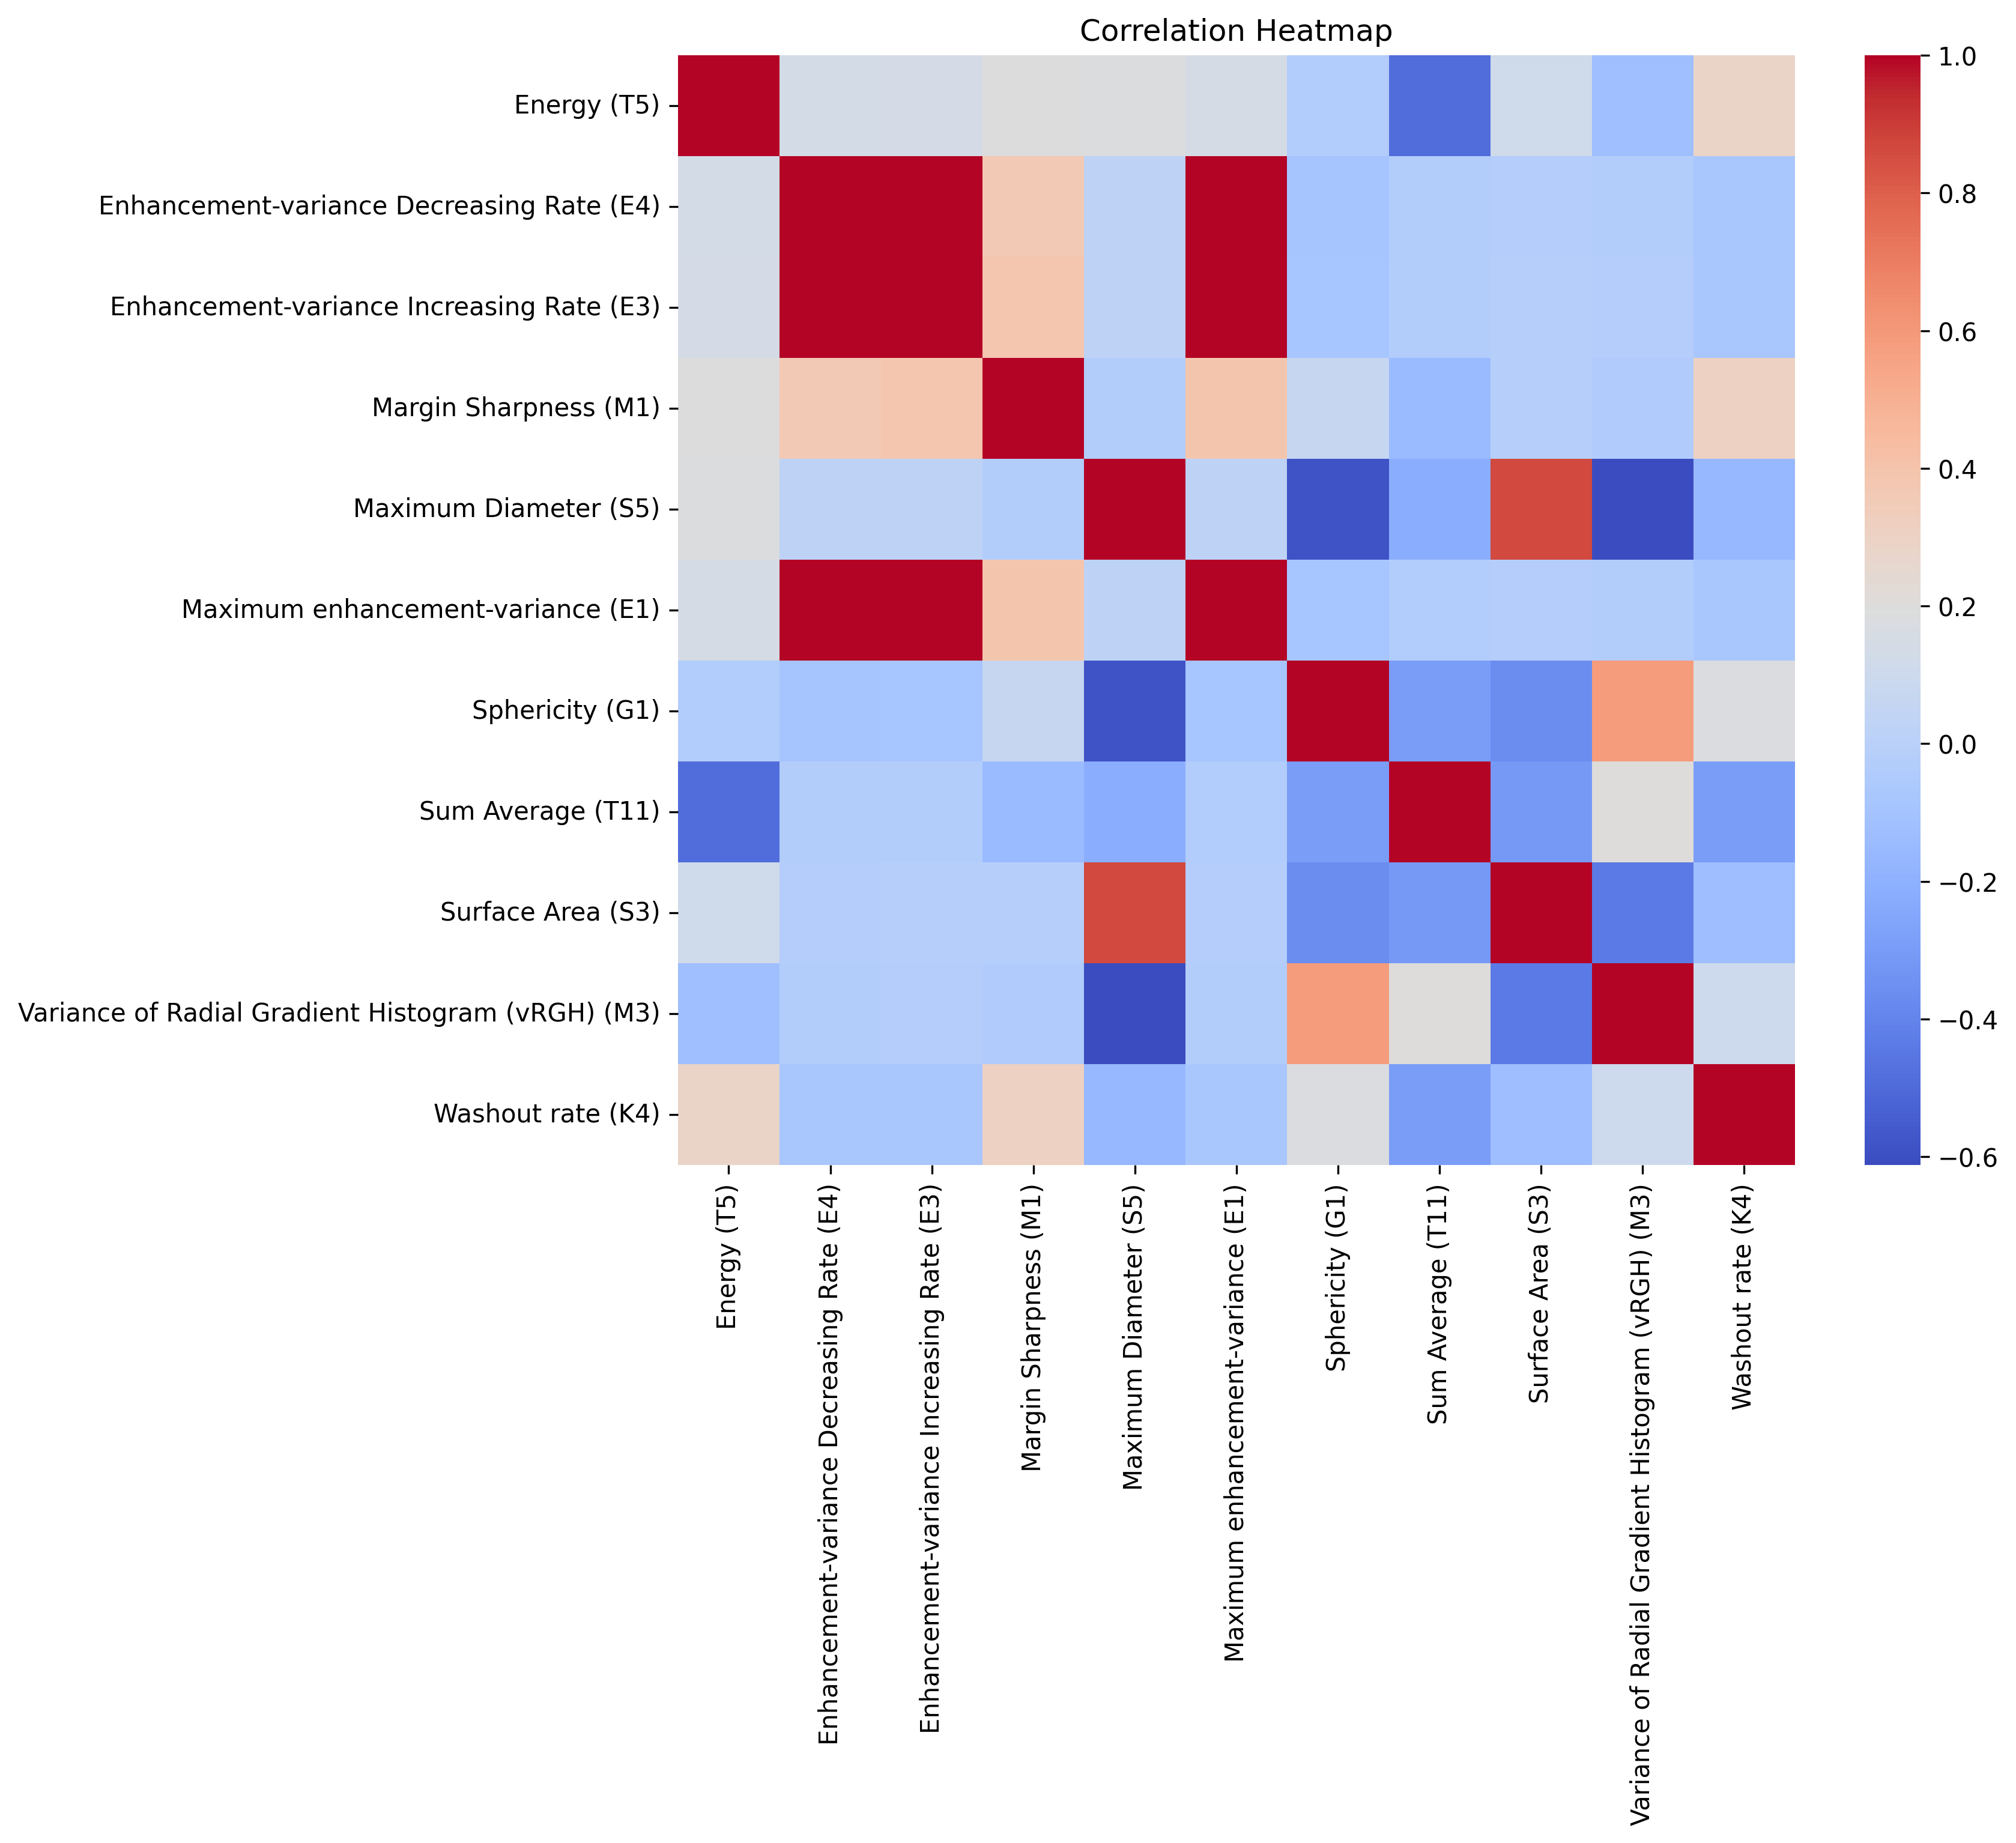
\includegraphics[width=0.5\textwidth]{images/correlation_heatmat.png}
    \caption{Correlation heatmap displaying the pairwise correlations between the selected features.}
    \label{fig:correlation_heatmap}
\end{figure}

\begin{figure}
    \centering
    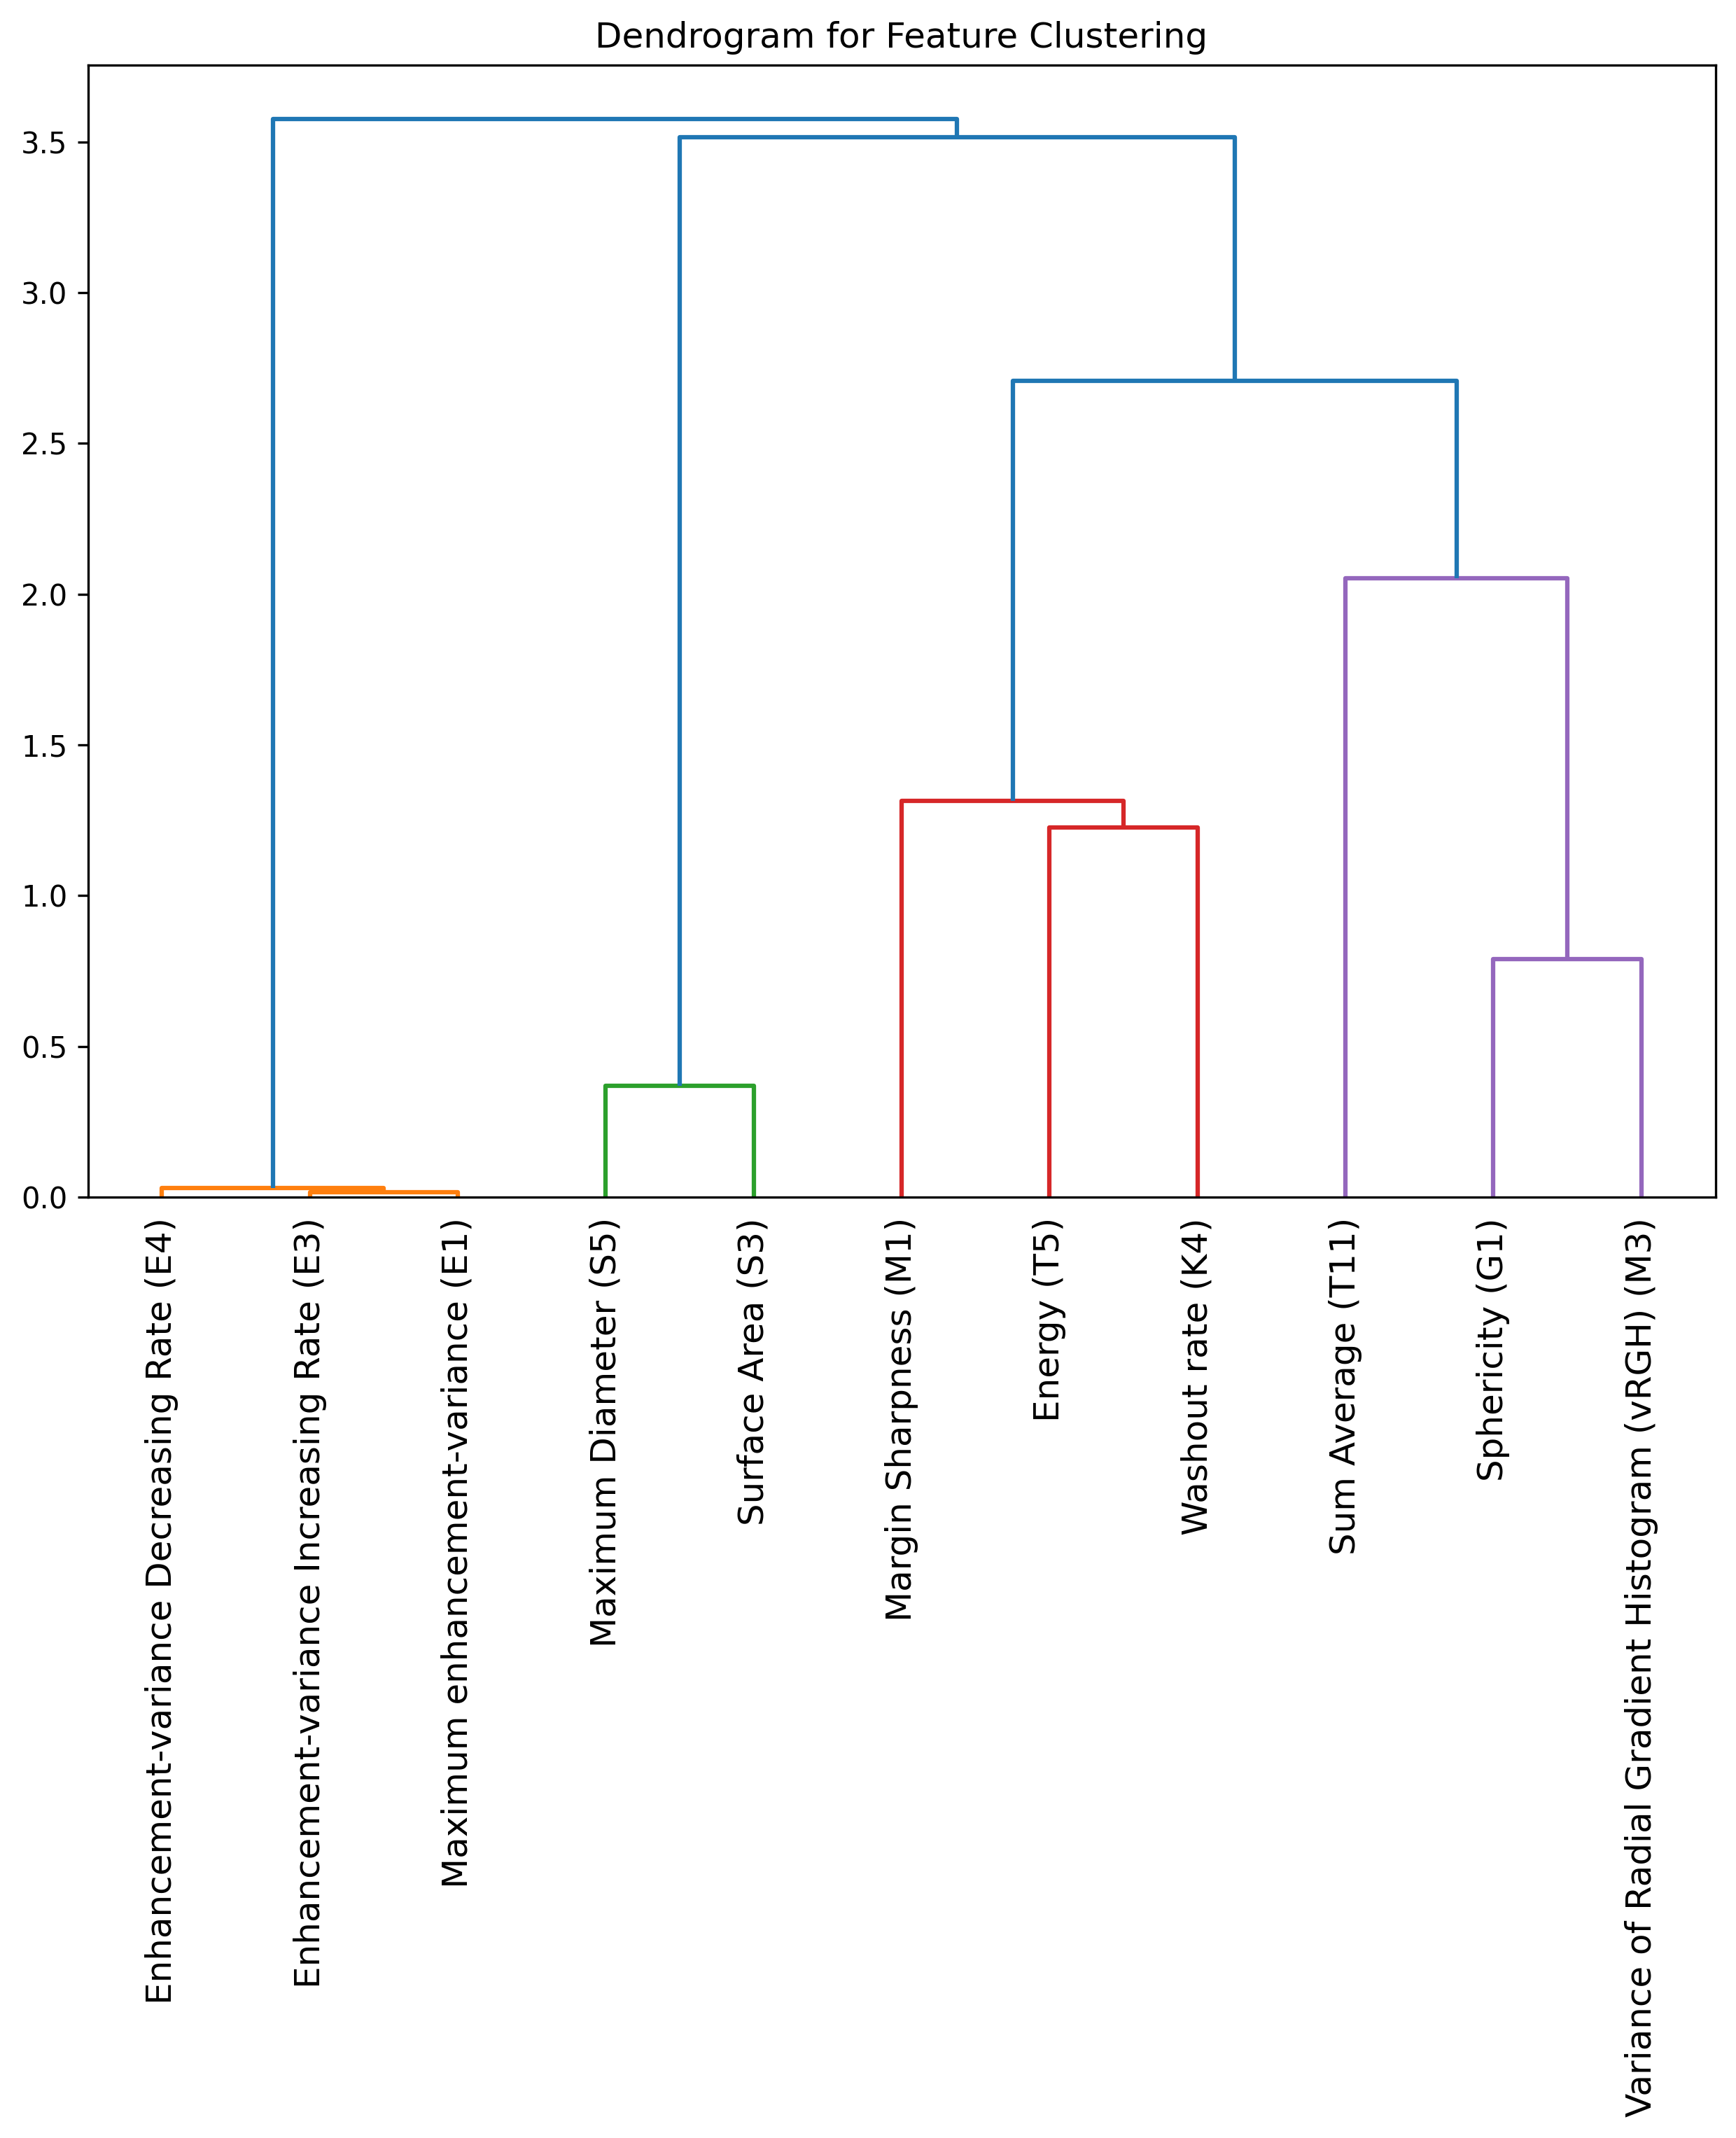
\includegraphics[width=0.45\textwidth]{images/dendrogram.png}
    \caption{Dendrogram resulting from hierarchical clustering}
    \label{fig:dendrogram}
\end{figure}

From these clusters, representative features were selected to reduce redundancy while retaining the most informative variables. After testing different numbers of clusters, it was determined that using three clusters provided a good balance without significantly affecting the model’s performance. The final representative features selected were:

\begin{itemize}
    \item \textbf{Margin Sharpness (M1)}. Describes the abruptness of intensity changes at the tumor’s boundary, indicating how clearly the tumor is demarcated from surrounding tissues. The sharpness is quantified by averaging the magnitude of the intensity gradient across all boundary voxels.

    \item \textbf{Maximum Enhancement-Variance (E1)}. Measures the variance in the enhancement signal across the most enhancing regions of the tumor, reflecting heterogeneity in vascularization.

    \item \textbf{Surface Area (S3)}. Represents the surface area of the tumor boundary, providing information about the tumor’s size and shape complexity. 
\end{itemize}

Finally, a Random Forest classifier was trained using the selected features obtained from the clustering process.

\subsubsection{Radiomic model with clinical data}

To evaluate the impact of clinical variables on the predictive performance of the model, two versions of the radiomic model were created by adding clinical data to the selected radiomic features:

\begin{itemize}
    \item \textbf{Full clinical data model}: This model incorporates the following clinical variables:
    \begin{itemize}
        \item \textbf{Age at diagnosis}
        \item \textbf{Cancer stage and tumor size}
        \item \textbf{Number of affected lymph nodes}
        \item \textbf{Hormone receptor status (estrogen and progesterone)}
    \end{itemize}
    
    \item \textbf{Reduced clinical data model}: This model excludes the hormone receptor status variables to avoid an overly optimistic evaluation. Clinically, these hormone receptor statuses are highly correlated with the molecular subtype, particularly in distinguishing Luminal A and Luminal B. Removing them allows the model to focus on more indirect clinical features and ensures that the predictions are not dominated by highly correlated variables.
\end{itemize}

In both cases, the selected radiomic features obtained from the clustering process—Margin Sharpness (M1), Maximum enhancement-variance (E1), and Surface Area (S3)—were combined with the clinical variables, and a Random Forest classifier was trained. 


\subsubsection{Radiomic model with multigenic assays}

To evaluate the impact of genomic information on the model’s performance, a radiomic model was created by incorporating multigenic assay variables. The selected radiomic features were combined with the following genomic variables:

\begin{itemize}
    \item \textbf{GHI\_RS Score}
    \item \textbf{Correlation with good outcome signature}
    \item \textbf{Proliferation-related gene expression}
\end{itemize}

A Random Forest classifier was trained on this combined feature set.

\subsection{Evaluation metrics used} \label{f1}

Given the significant class imbalance in the dataset, the macro F1-score was chosen as the primary evaluation metric. The macro F1-score calculates the F1-score for each class independently and then averages them, giving equal importance to each class, regardless of its frequency in the dataset. This is particularly useful in scenarios where some classes (such as Luminal A) are overrepresented, ensuring that the model's performance is not biased toward the majority class.

The F1-score for a single class is defined as the harmonic mean of precision and recall:

\begin{equation}
\text{F1} = 2 \times \frac{\text{Precision} \times \text{Recall}}{\text{Precision} + \text{Recall}}
\end{equation}

where:
\begin{itemize}
    \item \textbf{Precision}: The proportion of true positive predictions out of all predicted positives for a class.
    \item \textbf{Recall}: The proportion of true positive predictions out of all actual positives for a class.
\end{itemize}

The macro F1-score is then computed as:

\begin{equation}
\text{F1}_{\text{macro}} = \frac{1}{C} \sum_{i=1}^{C} \text{F1}_i
\end{equation}

where $C$ is the number of classes, and $\text{F1}_i$ is the F1-score for class $i$.

\subsection{Model performance results}

All the models described in Section \ref{models}, including an additional model trained with all features (radiomic, clinical, and multigenic data), as well as models trained using only clinical data and only multigenic assays (without radiomic features), were evaluated using the metric explained in Section \ref{f1}. The results of this evaluation are presented in Table \ref{tab:model_performance}.

\begin{table}
\centering
\begin{tabular}{lcc}
\hline
\textbf{Model} & \textbf{Accuracy} & \textbf{F1-score} \\
\hline
Only Radiomic & 0.62 & 0.45 \\
Radiomic + Reduced clinical data & 0.56 & 0.42 \\
Radiomic + Full clinical data & 0.75 & 0.78 \\
Radiomic + Multigenic & 0.81 & 0.74 \\
All (Radiomic + Full clinical + Multigenic) & 0.75 & 0.60 \\
Only full clinical data & 0.67 & 0.40 \\
Only Multigenic & 0.75 & 0.60 \\
\hline
\end{tabular}
\vspace{3mm}
\caption{Performance results for the different models based on accuracy and macro F1-score.}
\label{tab:model_performance}
\end{table}

%%%%%%%%%%%%%%%%%%%%%%%%%%%%%%%%%%%%%%%%%%%%%%%%%%%%%%%%%%%%%%%%%%%%%%%%%%%%%%%
%                                                                                              Results and discussion                                                                                                      %
%%%%%%%%%%%%%%%%%%%%%%%%%%%%%%%%%%%%%%%%%%%%%%%%%%%%%%%%%%%%%%%%%%%%%%%%%%%%%%%

\section{Results and discussion}

\subsection{Comparison of model performance}

The performance comparison across the different models, as shown in Table~\ref{tab:model_performance}, highlights significant differences based on the type of features included. The model using only radiomic features achieved a macro F1-score of 0.45, indicating limited predictive power. The highest performance (macro F1-score of 0.78) was observed for the radiomic features combined with full clinical data, showcasing the importance of including relevant clinical variables. Interestingly, the ``All" model, which includes radiomic, clinical, and multigenic data, did not surpass the radiomic + multigenic model, suggesting potential redundancy or noise when combining all feature sets.

\subsection{Impact of clinical data inclusion}

The inclusion of clinical data, particularly hormone receptor status and tumor staging information, significantly enhanced the performance of the radiomic model. The Radiomic + Full clinical data model, which included hormone receptor status variables, achieved an F1-score of 0.78. In contrast, the Radiomic + Reduced clinical data model, excluding these variables to avoid optimistic bias, had a lower F1-score of 0.42. This outcome confirms the predictive value of hormone receptor status in distinguishing molecular subtypes.

\subsection{Impact of multigenic assays on prediction}

The addition of genomic data from multigenic assays further enhanced the model’s performance. The Radiomic + Multigenic model achieved an F1-score of 0.74, outperforming the radiomic-only model and the clinical-only models. Notably, the Only Multigenic model achieved a comparable F1-score of 0.60, indicating that genomic features alone can provide substantial predictive power. However, when combined with radiomic features, the predictive accuracy improved, suggesting that radiomic data provide complementary information about tumor phenotype that is not captured by genomic assays alone. This finding supports the integration of imaging and genomic data for more robust subtype classification.

\subsection{Detailed Performance of the Best Model}

Due to the strong performance of the Radiomic + Full clinical data model, we consider it relevant to explore its performance using the confusion matrix from the test set. As shown in Figure~\ref{fig:confusion_matrix}, the model accurately predicts the Basal and HER2-enriched subtypes, demonstrating reliable classification for these categories. However, it tends to confuse Luminal A and Luminal B subtypes, as evidenced by the misclassification of several Luminal A instances as Luminal B.

\begin{figure}[H]
    \centering
    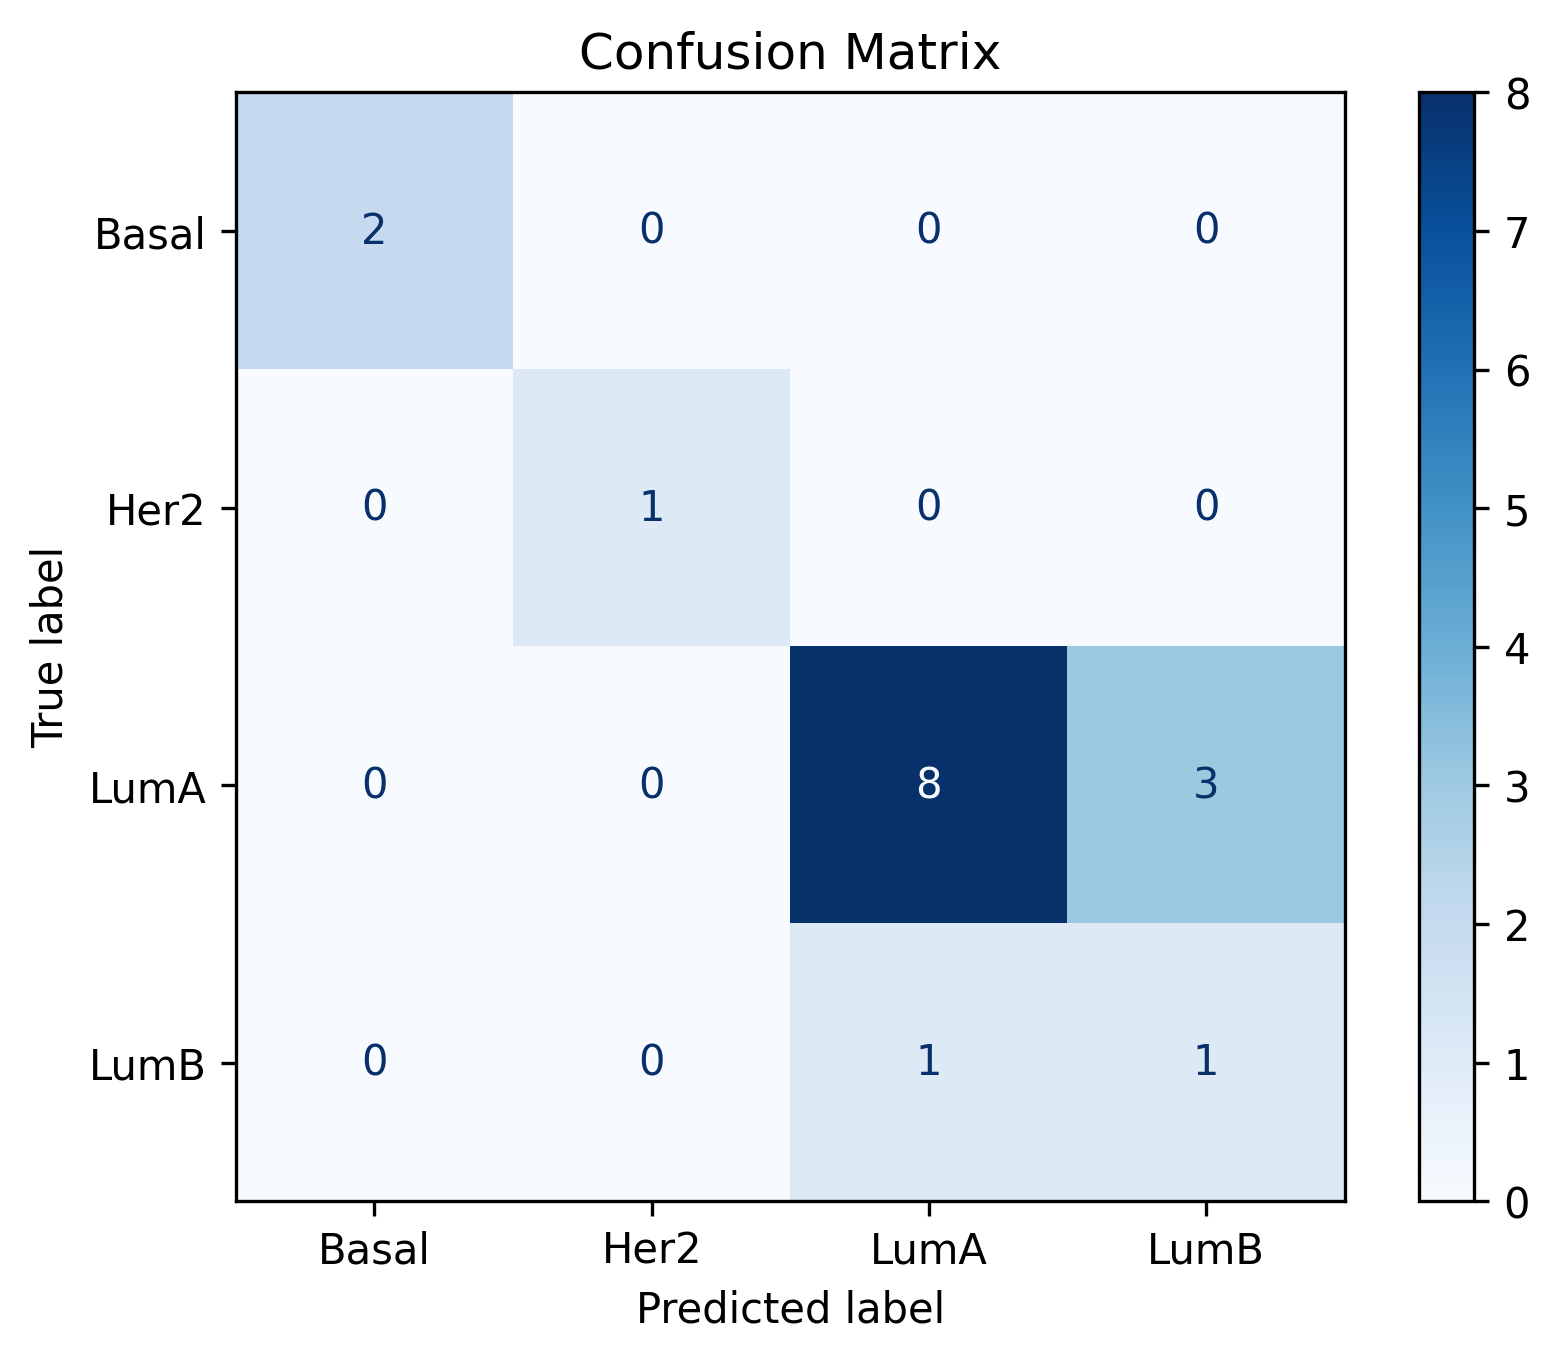
\includegraphics[width=0.4\textwidth]{images/confusion_matrix.png}
    \caption{Confusion matrix for the \textbf{Radiomic + Full clinical data} model.}
    \label{fig:confusion_matrix}
\end{figure}


%%%%%%%%%%%%%%%%%%%%%%%%%%%%%%%%%%%%%%%%%%%%%%%%%%%%%%%%%%%%%%%%%%%%%%%%%%%%%%%
%                                                                                                               CONCLUSION                                                                                                 %
%%%%%%%%%%%%%%%%%%%%%%%%%%%%%%%%%%%%%%%%%%%%%%%%%%%%%%%%%%%%%%%%%%%%%%%%%%%%%%%
 
\section{Conclusions}

\subsection{Key findings}

This study demonstrated that combining radiomic, clinical, and genomic data enhances the prediction of molecular subtypes of breast cancer. The Radiomic + Full clinical data model achieved the highest performance, with an F1-score of 0.78, highlighting the importance of hormone receptor status and other clinical variables in subtype classification. The inclusion of multigenic assays also improved the model’s performance, with the Radiomic + Multigenic model achieving an F1-score of 0.74, showing the complementarity between genomic data and radiomic features. However, the ``All'' model did not outperform the others, suggesting potential redundancy and the need for careful feature selection.

\subsection{Study limitations}

Several limitations should be acknowledged:
\begin{itemize}
    \item \textbf{Small dataset size}: The number of instances available for training and evaluation was limited, which may have impacted the model’s generalizability and robustness.
    \item \textbf{Limited computational resources}: The complexity of feature selection and model training was constrained by computational resources, potentially limiting the exploration of more advanced model architectures or hyperparameter optimization.
\end{itemize}

\subsection{Suggestions for future work}

Future work could address these limitations through the following actions:
\begin{itemize}
    \item \textbf{Increased data collection}: Incorporating more patient data, especially from diverse cohorts, would improve model generalization and allow for a more accurate evaluation.
    \item \textbf{Better data organization and integration}: A more structured approach to organizing radiomic, clinical, and genomic data would facilitate preprocessing, feature extraction, and model training, potentially improving performance and interpretability.
    \item \textbf{Extraction of radiomic features from raw images}: Performing feature extraction directly from the original MRI scans would allow for a more customized approach and could uncover more relevant imaging biomarkers.
    \item \textbf{Hyperparameter tuning}: Future studies should focus on optimizing hyperparameters such as learning rate, number of estimators, and regularization parameters to improve model performance and reduce overfitting.
\end{itemize}

%%%%%%%%%%%%%%%%%%%%%%%%%%%%%%%%%%%%%%%%%%%%%%%%%%%%%%%%%%%%%%%%%%%%%%%%%%%%%%%
%                                                                                                        REFERENCES                                                                                                          %
%%%%%%%%%%%%%%%%%%%%%%%%%%%%%%%%%%%%%%%%%%%%%%%%%%%%%%%%%%%%%%%%%%%%%%%%%%%%%%%

\begin{thebibliography}{00}

\bibitem{breast_cancer} World Health Organization. "Cancer: Fact Sheets." Available: https://www.who.int/news-room/fact-sheets/detail/cancer. [Accessed: Jan. 5, 2025].

\bibitem{b1} Komen, S. Foundation. Molecular Subtypes of Breast Cancer. Komen.org. Available at: https://www.komen.org/breast-cancer/diagnosis/molecular-subtypes (Accessed January 4, 2025).

\bibitem{b2} Saha A, Harowicz MR, Grimm LJ, Kim CE, Ghate SV, Walsh R, Mazurowski MA. A machine learning approach to radiogenomics of breast cancer: a study of 922 subjects and 529 DCE-MRI features. Br J Cancer. 2018 Aug;119(4):508-516. doi: 10.1038/s41416-018-0185-8. Epub 2018 Jul 23. PMID: 30033447; PMCID: PMC6134102.

\bibitem{b3} Morris, E., Burnside, E., Whitman, G., Zuley, M., Bonaccio, E., Ganott, M., Sutton, E., Net, J., Brandt, K., Li, H., Drukker, K., Perou, C., \& Giger, M. L. (2014). Using Computer-extracted Image Phenotypes from Tumors on Breast MRI to Predict Stage [Data set]. The Cancer Imaging Archive. https://doi.org/10.7937/K9/TCIA.2014.8SIPIY6G

\bibitem{b4} Brandt, J., Garne, J.P., Tengrup, I. et al. Age at diagnosis in relation to survival following breast cancer: a cohort study. World J Surg Onc 13, 33 (2015). https://doi.org/10.1186/s12957-014-0429-x

\bibitem{b5} Komen, S. Foundation. Factors that Affect Prognosis: Lymph Node Status. Komen.org. Available at: https://www.komen.org/breast-cancer/diagnosis/factors-that-affect-prognosis/lymph-node-status (Accessed January 5, 2025).

\bibitem{b6} Wikipedia. "Breast cancer classification." Available: https://en.wikipedia.org/wiki/Breast\_cancer\_classification. [Accessed: Jan. 5, 2025]

\bibitem{b7} Syed, Y.Y. Oncotype DX Breast Recurrence Score®: A Review of its Use in Early-Stage Breast Cancer. Mol Diagn Ther 24, 621–632 (2020). https://doi.org/10.1007/s40291-020-00482-7

\bibitem{b8} Wikipedia. "MammaPrint." Available: https://en.wikipedia.org/wiki/MammaPrint. [Accessed: Jan. 5, 2025].

\end{thebibliography}

\end{document}